\subsection{FLEX-IS (model ID: 34)}
The FLEX-IS model (fig.~\ref{fig:34_schematic}) is a combination of the FLEX-B model expanded with an interception (I) routine \citep{Fenicia2008} and a snow (S) module \citep{Nijzink2016}. It has 5 stores and 12 parameters ($TT$, $ddf$, $I_{max}$, $UR_{max}$, $\beta$, $L_p$, $Perc_{max}$, $D$, $N_{lag,f}$, $N_{lag,s}$, $K_f$ and $K_s$). The model aims to represent:

\begin{itemizecompact}
\item Snow accumulation and melt;
\item Interception by vegetation;
\item Infiltration and saturation excess flow based on a distribution of different soil depths;
\item A split between fast saturation excess flow and preferential recharge to a slow store;
\item Percolation from the unsaturated zone to a slow runoff store.
\end{itemizecompact}

\subsubsection{File names}
\begin{tabular}{@{}ll}
Model: &m\_34\_flexis\_12p\_5s \\
Parameter ranges: &m\_34\_flexis\_12p\_5s\_parameter\_ ranges \\
\end{tabular}

% Equations
\subsubsection{Model equations}

% Model layout figure
{ 																	% This ensures it doesn't warp text further down
\begin{wrapfigure}{l}{7cm}
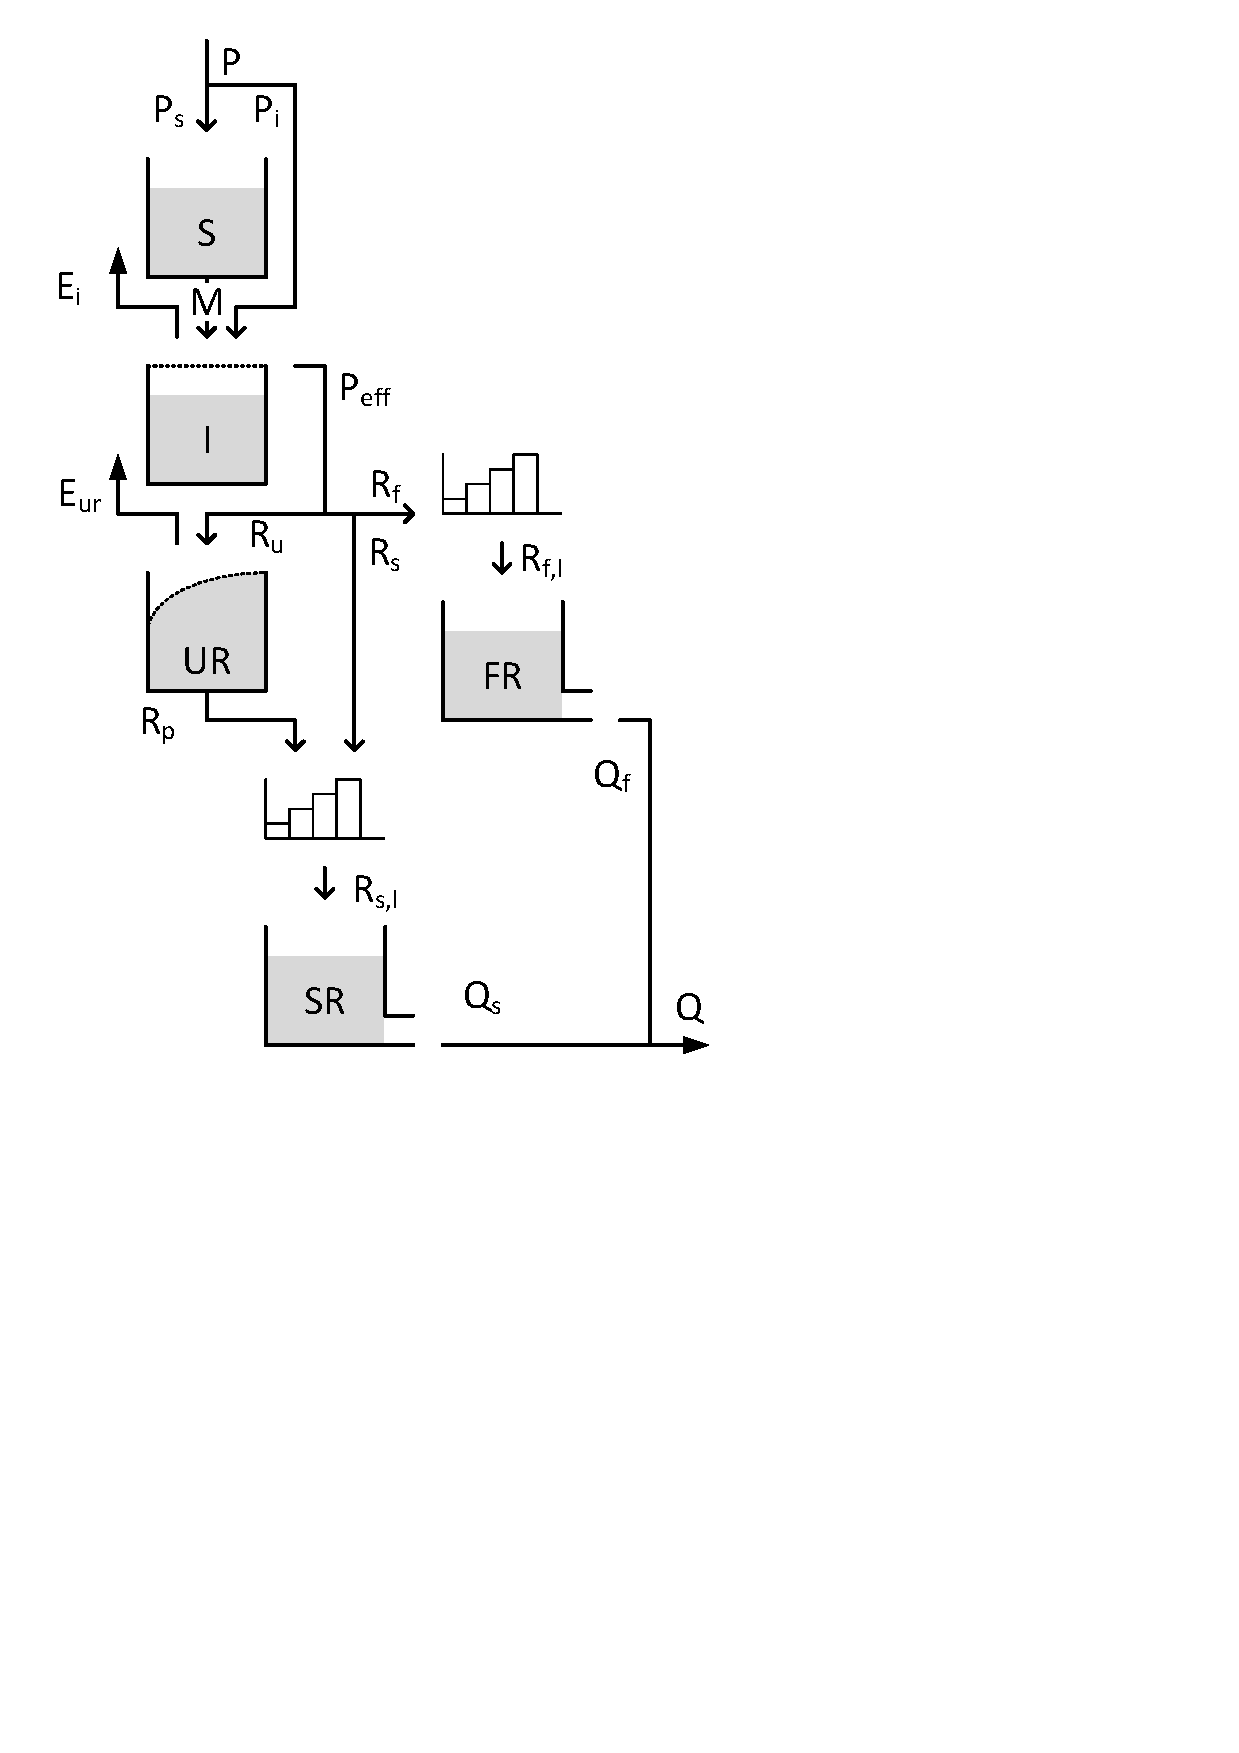
\includegraphics[trim=1cm 12cm 7cm 1cm,width=7cm,keepaspectratio]{./files/34_schematic.pdf}
\caption{Structure of the FLEX-IS model} \label{fig:34_schematic}
\end{wrapfigure}

\begin{align}
	\frac{dS}{dt} &= P_s-M \\
	P_s &= \begin{cases}
		P, &\text{if } T \leq TT \\
		0, & \text{otherwise} \\
	\end{cases} \\
	M &= 
	\begin{cases}
		ddf*(T - TT), & \text{if } T \geq TT \\
		0, & \text{otherwise}
	\end{cases}
\end{align}

Where S [mm] is the current snow storage, $P_s$ the precipitation that falls as snow [mm/d], M the snowmelt $[mm/d]$ based on a degree-day factor (ddf, [mm/\degree C/d]) and threshold temperature for snowfall and snowmelt (TT, [\degree C]).


\begin{align}
	\frac{dI}{dt} &= P_I + M - E_I  - P_{eff}\\
	P_i &= \begin{cases}
		P, &\text{if } T > TT \\
		0, & \text{otherwise} \\
	\end{cases} \\
	E_i &= \begin{cases}
		E_p, &\text{if } I > 0 \\
		0, &\text{otherwise} \\
	\end{cases} \\
	P_{eff} &= \begin{cases}
		P_i, &\text{if } I = I_{max}\\
		0, &\text{otherwise}\\
	\end{cases}	
\end{align}
} % end of wrapfigure fix
Where $P_I$  $[mm/d]$ is the incoming precipitation, I is the current interception storage [mm], which is assumed to evaporate ($E_i$ $[mm/d]$) at the potential rate $E_p$ $[mm/d]$ when possible. When I exceeds the maximum interception storage $I_{max}$ [mm], water is routed to the rest of the model as $P_{eff}$ $[mm/d]$. 

\begin{align}
	\frac{dUR}{dt} &= R_u - E_{ur} - R_p \\
	%R_U &= (1 - C_r) * P_{eff}\\
	%C_r &= \Big[1+exp\Big(\frac{-UR/UR_{max} + 1/2}{\beta}\Big)\Big]^{-1}\\
	R_u &= (1 - \Big[1+exp\Big(\frac{-UR/UR_{max} + 1/2}{\beta}\Big)\Big]^{-1}) * P_{eff}\\
	E_{ur} &= E_p * min\Big(1, \frac{UR}{UR_{max}} \frac{1}{L_p}\Big)\\
	R_p &= Perc_{max} * \frac{-UR}{UR_{max}}
\end{align}
  
Where UR is the current storage in the unsaturated zone [mm]. $R_u$  $[mm/d]$ is the inflow into UR based on its current storage compared to maximum storage $UR_{max}$ [mm] and a shape distribution parameter $\beta$ [-]. $E_{ur}$ the evaporation $[mm/d]$ from UR which follows a linear relation between current and maximum storage until a threshold $L_p$ [-] is exceeded. $R_p$ $[mm/d]$ is the percolation from UR to the slow reservoir SR [mm], based on a maximum percolation rate $Perc_{max}$ $[mm/d]$, relative to the fraction of current storage and maximum storage.

\begin{align}
	R_s &= (P_{eff} - R_u)*D\\
	R_f &= (P_{eff} - R_u)*(1-D)
\end{align}

Where $R_s$ and $R_f$ are the flows $[mm/d]$ to the slow and fast runoff reservoir respectively, based on runoff partitioning coefficient D [-]. Both are lagged by linearly increasing triangular transformation functions with parameters $N_{lag,s}$ and $N_{lag,f}$ respectively, that give the number of time steps over which $R_s$ and $R_f$ need to be transformed. $R_p$ is added to $R_s$ before the transformation occurs.

\begin{align}
	\frac{dFR}{dt} &= R_{f,l} - Q_f\\
	Q_f &= K_f * FR 
\end{align}

Where FR is the current storage [mm] in the fast flow reservoir. Outflow $Q_f$ $[mm/d]$ from the reservoir has a linear relation with storage through time scale parameter $K_f$ [$d^{-1}$]. 

\begin{align}
	\frac{dSR}{dt} &= R_{s,l} - Q_s \\
	Q_s &= K_s * SR 
\end{align}

Where SR is the current storage [mm] in the slow flow reservoir. Outflow $Q_s$ $[mm/d]$ from the reservoir has a linear relation with storage through time scale parameter $K_s$ [$d^{-1}$]. 

\begin{align}
	Q = Q_f + Q_s
\end{align}

Where Q $[mm/d]$  is the total simulated flow as the sum of $Q_s$ and $Q_f$.

\subsubsection{Parameter overview}
% Table generated by Excel2LaTeX from sheet 'Sheet1'
\begin{table}[htbp]
  \centering
    \begin{tabular}{lll}
    \toprule
    Parameter & Unit  & Description \\
    \midrule
    $TT$  & $^oC$ & Threshold temperature for snowfall and melt \\
    $ddf$ & $mm~^oC^{-1}~d^{-1}$ & Degree-day factor \\
    $I_{max}$ & $mm$  & Maximum interception storage \\
    $UR_{max}$ & $mm$  & Maximum soil moisture storage \\
    $\beta$ & $-$   & Shape parameter \\
    $L_p$ & $-$   & Wilting point as fraction of $UR_{max}$ \\
    $Perc_{max}$ & $mm~d^{-1}$ & Maximum percolation rate \\
    $D$   & $-$   & Fraction effective precipitation to slow store \\
    $N_{lag,f}$ & $d$   & Unit Hydrograph time base \\
    $N_{lag,s}$ & $d$   & Unit Hydrograph time base \\
    $K_f$ & $d^{-1}$ & Runoff coefficient \\
    $K_s$ & $d^{-1}$ & Runoff coefficient \\
    \bottomrule
    \end{tabular}%
  \label{tab:addlabel}%
\end{table}%

